\documentclass{beamer}

% Theme choice (you can change to Madrid, CambridgeUS, etc.)
\usetheme{Madrid}

% Optional packages
\usepackage[utf8]{inputenc}
\usepackage{graphicx} % for including images
\usepackage{amsmath, amssymb, mathtools} % for math symbols
\usepackage{hyperref} % for clickable links
\usepackage{tikz}

% Title info
\title[Short Title]{Factor Models of Returns}
\author[Your Name]{Oden Petersen}
\date{\today}

% Section headers
\AtBeginSection[]{
	\begin{frame}
	\vfill
	\centering
	\begin{beamercolorbox}[sep=8pt,center,shadow=True,rounded=True]{title}
		\usebeamerfont{title}\insertsectionhead\par%
	\end{beamercolorbox}
	\vfill
	\end{frame}
}

\begin{document}

% Title page
\begin{frame}
	\titlepage
	\begin{center}
		\textit{``$y=X\beta+\epsilon$, the rest is commentary.''}
	\end{center}
\end{frame}

\begin{frame}{About Me}
\end{frame}

% Table of contents
\begin{frame}{Outline}
	\tableofcontents
	%% Good to include concrete data examples throughout
\end{frame}

% Section 1
\section{Securities Markets}

\begin{frame}{Spot Transactions}
	The point of trading is to obtain an asset by giving up money, or obtain money by giving up an asset.

	If I give you $q$ units of some asset $A$, and you give me $\$p$, then:
	\begin{itemize}
		\item I have \textbf{sold} $q$ units of $A$ to you at $\frac{\$p}{q}$
		\item You have \textbf{bought} $q$ units of $A$ from me for $\frac{\$p}{q}$
	\end{itemize} %"for" and "at" indicate direction

	Buying and selling are collectively called `trading'.

	Suppose I own some amount of $A$ and some amount of money. If we let $s$ be $+1$ for buying and $-1$ for selling, then the result of any trade is to add $qs$ to the amount of $A$ I own, and add $-qps$ to the amount of money I have. %s is called the sign of the trade

	% Stock image of retail store
\end{frame}

\begin{frame}{Securities Markets and Exchanges}
	The \textbf{\textcolor{blue}{market}} is the collective activity of all traders. When we don't care who we trade with, we can just `trade with the market'.

	A \textbf{\textcolor{red}{securities} \textcolor{blue}{market}} for some asset $A$, open at a time $t$, is any \textcolor{red}{standardised} \textcolor{blue}{way for traders to reach agreements to buy or sell} $A$ at a specified \textbf{settlement time} $T\geq t$. %"securities" because of standardisation and regulation

	\pause

	For example, $T=\ldots$
	\begin{itemize}
		\item $t$ (`spot', e.g. blockchain) %ASX tried to do blockchain, this was scrapped in 2022 after 7yrs
		\item $t+1, t+2, \ldots$ (`clearing', e.g. equities)
		\item Last Thursday of month (`futures')
	\end{itemize}

	\pause
	If you agree to give something to someone, you have an \textbf{obligation}. If someone agrees to give you something, you have a \textbf{right}.

	\begin{block}{Counterparty Risk}
		If I have an agreement with $P_1$ to buy $10$ units for $\$p_1$ at $T$, and an agreement with $P_2$ to sell $10$ units at $\$p_2$ at $T$, and no further rights/obligations, am I guaranteed to meet my obligations?
	\end{block}%Define counterparty risk
\end{frame}

\begin{frame}{Centralisation}
	A \textbf{securities exchange} is a centralised venue serving a securities market for \textbf{exchange participants} (e.g. ASX, NYSE, TSE, HKEX, LME).

	Agreements not made through an exchange are often called OTC (over-the-counter). %Also called off-exchange. Define search costs.

	\begin{center}
		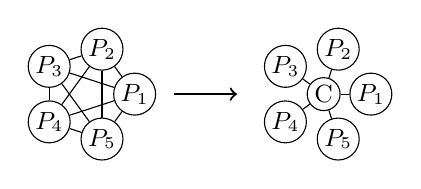
\begin{tikzpicture}[baseline, every node/.style={circle, draw, fill=white, inner sep=1pt, font=\small, minimum size=1mm}]
			\foreach \i in {1,...,5} {
				\node (n\i) at ({72*(\i-1)}:0.6) {$P_{\i}$};
			}
			\foreach \i in {1,...,5} {
				\foreach \j in {1,...,5} {
					\ifnum\i<\j
						\draw (n\i) -- (n\j);
					\fi
				}
			}

			\draw[->, thick] (1.1,0) -- (1.9,0);

			\begin{scope}[xshift=3cm]
				\node (c) at (0,0) {C};
				\foreach \i in {1,...,5} {
					\node (n\i) at ({72*(\i-1)}:0.6) {$P_{\i}$};
					\draw (c) -- (n\i);
				}
			\end{scope}
		\end{tikzpicture}
	\end{center}

	Centralisation generally reduces \textbf{search costs} and \textbf{counterparty risk}. %Mention risk counterexample: FTX vs a DEX
\end{frame}

\begin{frame}{Settlement and Clearing}
	\begin{block}{Netting}
		Centralisation allows for \textbf{netting} of rights and obligations.

		For any settlement time $T$, I only need to keep track of the difference between money owed to and by me, and units owed to and by me.

		The quantity of $A$ owned by me, plus the quantity owed to me, minus the quantity owed by me to others, is known as my \textbf{net position} in $A$. If this is positive, I have a \textbf{long position}. If it is negative, I have a \textbf{short position}. If it is zero, I am \textbf{flat}.
	\end{block}

	\begin{block}{Collateralisation}
		At certain intermediate times $t'$ ($t\leq t'\leq T$), participants may be required to physically give (`post') something to the exchange to \textbf{collateralise} their obligations.
		\begin{itemize}
			\item Money (`margin') %Explain the term "futures type settlement" and "stock type settlement"
			\item Assets (`locate'/`borrow') %"Borrow" is only if you don't own the thing
		\end{itemize}
		If an agreement made on the exchange gives you rights to money or assets, this is typically as good as posting actual money or assets.
	\end{block}
\end{frame}

\begin{frame}{Summary}
	\begin{itemize}
		\item \textbf{Trading} is swapping money and assets
		\item A \textbf{market} is whatever you use to trade
		\item A \textbf{securities market} is a standardised way to agree to trades
		\item Agreements consist of \textbf{rights} and \textbf{obligations}
		\item Finding a \textbf{counterparty} may involve \textbf{search cost}
		\item Agreements between two parties are subject to \textbf{counterparty risk}
		\item A \textbf{securities exchange} is a centralised trading venue %Maybe explain national market system
		\item After trades are agreed to on an exchange, they will be \textbf{settled} in some standardised way
		\item The net quantity of $A$ I have some claim to can either be positive (\textbf{long position}), negative (\textbf{short position}), or zero (\textbf{flat}).
		\item Traders may be obligated to post assets ('locate') or money ('margin')
	\end{itemize}
\end{frame}

\section{Trading}
\begin{frame}{Setup}
	A sequence of trades that collectively increases the amount of money you have and leaves the amount of each asset you have unchanged is clearly favourable.

	\pause

	Suppose that at each time $t$ we have cash holdings of $\$c_t$ and net holdings of $a_t$ units of some asset $A$.

	Suppose also that trades $(s_t, q_t, \$p_t)$ take place at a finite set of distinct times
	$$\tau = \{t_1,\ldots t_n\}\subset T = [t_-, t_+],$$
	where $t_-<t_1<\ldots<t_n<t_+$.

	\pause

	Suppose further that $p_t$ is a right-continuous function $\mathbb R\to\mathbb R$ with left-limits.

	For instance, we could take $p_t = p_{\max \left(\tau\cap (-\infty,t]\right)}$ for $t\geq \min\tau$ and $p_t=x$ otherwise for some arbitrary $x$. %Last traded price

\end{frame}

\begin{frame}{Accounting}
	Let $c_t^+, a_t^+, p_t^+$ be the right-limits and $c_t^-, a_t^-, p_t^-$ the left-limits of $c_t,a_t, p_t$ respectively.

	\pause

	\textcolor{blue}{Define measures $a_\omega, c_\omega, p_\omega$ such that for any interval $T'=[t_-',t_+']$ we have}

	\vspace{-0.06\textheight}
	\begin{align*}
		\textcolor{blue}{a_{T'}} &&= \int_{T'} da &&= a_{t_+'}^+ - a_{t_-'}^-
	\\	\textcolor{blue}{c_{T'}} &&= \int_{T'} dc &&= c_{t_+'}^+ - c_{t_-'}^-
	\\	\textcolor{blue}{p_{T'}} &&= \int_{T'} dp &&= p_{t_+'}^+ - p_{t_-'}^- &&= p_{t_+'} - p_{t_-'}^-.
	\end{align*}%Special case: t_-'=t_+'

	\pause

	Then we have
	\vspace{-0.04\textheight}
	\begin{align*}
		\textcolor{blue}{a_T}	&&= a_{t_+}^+ - a_{t_-}^- 	&= \sum_{t\in \tau} s_t q_t		&&= \int_{t\in T} da,
	\\	\textcolor{blue}{c_T}	&&= c_{t_+}^+ - c_{t_-}^- 	&= \sum_{t\in \tau} - p_t (s_t q_t)	&&= \int_{t\in T} - p_t da,
	\\	\textcolor{blue}{p_T}	&&= p_{t_+}^+ - p_{t_-}^- 	&= p_{t_+} - p_{t_-'}^-			&&= \int_{t\in T} dp.
	\end{align*}
\end{frame}

\begin{frame}{Cash Holdings}
	\vspace{-0.15\textheight}
	\begin{align*}
		\\	c_{t_+} - c_{t_-}	&= \sum_{t\in\tau} - p_t (s_t q_t)	&&= \sum_{i=1}^n - p_{t_i} (a_{t_i}^+-a_{t_i}^-) = - \sum_{i=1}^n p_{t_i} a_{t_i}^+ + \sum_{i=1}^n p_{t_i} a_{t_i}^-
		\\				&					&&= - \sum_{i=1}^{n-1} p_{t_i} a_{t_{i+1}}^- - p_{t_n} a_{t_n}^+ + \sum_{i=1}^{n-1} p_{t_{i+1}} a_{t_{i+1}}^- + p_{t_1}a_{t_1}^-
		\\				&					&&= p_{t_1}a_{t_1}^- + - p_{t_n} a_{t_n}^+ + \sum_{i=2}^n (p_{t_i}-p_{t_{i-1}}) a_{t_i}^-
		\\				&					&&\textcolor{blue}{= p_{t_1}a_{t_1}^- - p_{t_n}a_{t_n}^+ + \int_{t\in[t_1,t_n]} a_t^- dp},
		\\				&					&&\textcolor{blue}{= p_{t_-}a_{t_-} - p_{t_+}a_{t_+} + \int_{t\in T} a_t^- dp},
	\end{align*}
	This is similar in spirit to integration by parts:
	$$\int_a^b f \frac{dg}{dx} dx = f(b)g(b)-f(a)g(a) - \int_a^b g \frac{df}{dx} dx.$$
\end{frame}

\begin{frame}{Accounting Summary}
	\begin{align*}
		a_{t_+}^+ - a_{t_-}^-	&= \int_{t\in T} da,
	\\	c_{t_+}^+ - c_{t_-}^- 	&= \int_{t\in T} - p_t da,
	\\	p_{t_+}^+ - p_{t_-}^- 	&= \int_{t\in T} dp		&= p_{t_-}a_{t_-} - p_{t_+}a_{t_+} + \int_{t\in T} a_t^- dp.
	\end{align*}
\end{frame}

\begin{frame}{Portfolio Valuation}
	Then we have
	$$(c_{t_+} + p_{t_+}a_{t_+}) - (c_{t_-} + p_{t_-}a_{t_-}) = \int_{t\in T} a_t^- dp.$$

	The quantity $\$v_t = \$p_t a_t$ is known as the \textbf{dollar value} of our $A$ holdings \textbf{marked} to the price $\$p_t$.

	\pause

	Suppose now that we trade multiple assets, such that $p_t$, $a_t$ and $v_t$ are vector-valued, with $v_t$ the elementwise product of $p_t$ and $a_t$.

	A collection of assets held in quantities $a_t$ is known as a \textbf{portfolio}.

	We can write
	$$(c_{t_+} + p_{t_+} \cdot a_{t_+}) - (c_{t_-} + p_{t_-} \cdot a_{t_-}) = \int_{t\in T} a_t^- \cdot dp,$$
	where $p$ is now a vector-valued measure. \pause Let
	$$\Pi_t	= c_t + p_t\cdot a_t = c_t + \sum v_t.$$

	We call $\$\Pi_t$ the \textbf{value} of our portfolio \textbf{marked} to $p_t$.
\end{frame}

\begin{frame}{Profitability}
	The quantity $\$\Pi_{t_+} - \$\Pi_{t_-}$ is our \textbf{net P\&L} (profit and loss) over the interval $T$, marked to $p_t$.
	Then we have
	$$\Pi_{t_+} - \Pi_{t_-} = \int_{t\in T} a_t^- \cdot dp,$$
	and \textcolor{blue}{defining $\Pi_{T'} = \Pi_{t_+'}^+ - \Pi_{t_-'}^-$ as before,} we can write
	$$\textcolor{blue}{\Pi_{[t_i,t_{i+1}]}} = \int_{t\in [t_i, t_{i+1}]} d\Pi = a_t^- \cdot dp = \int_{t\in [t_i, t_{i+1}]} v_t^- \cdot \frac{dp}{p_t^-},$$
	where $\frac{dp}{p_t^-}$ is the elementwise quotient.

	Furthermore, we can write
	$$\frac{\int_T d\Pi}{\Pi_t^-} = \frac{1}{\Pi_t^-}v_t^- \cdot \frac{dp}{p_t^-} = w_t^- \cdot \frac{dp}{p_t^-},$$
	where $w_t = \frac{1}{\Pi_t}v_t$ is the \textbf{weight vector}. %Explain the interpretation of this
\end{frame}

\begin{frame}{Leverage}
	Suppose we can always make any trade we like at time $t$ with price $\$p_t$.

	Then we can freely convert a portfolio with value $\$\Pi_t$ to that much in cash.

	Conversely, we can convert $\$\Pi_t$ worth of cash into any portfolio with that value.

	In practice, there are limits on the trades we can make at a particular price and time.

	\pause

	Typically, $\Pi_t$ can change in two ways: trading assets, or transferring cash into and out of the portfolio. We will generally ignore the possibility of transfers.

	\pause

	If we begin with a portfolio worth $\$\Pi_{t_1}$ and make a sequence of trades of the form $(s_t,q_t,p_t)$ that result in a portfolio worth $\$\Pi_{t_n}$, then we could instead begin with a portfolio worth $L \$\Pi_{t_1}$ and make trades $(s_t, L q_t, p_t)$ to arrive at a portfolio worth $L \$\Pi_{t_n}$. The ratio $L$ is known as the \textbf{leverage ratio}.
\end{frame}

\begin{frame}{Returns}
	Because cash kept in a portfolio cannot be put to use elsewhere, we might want an estimate for how much extra P\&L would result from a marginal dollar added to the portfolio value over the interval $T$.

	If our initial portfolio value were $\$\Pi_{t_-}+\$1$ instead of $\Pi_{t_-}$, and we can simply scale up trade sizes at the same prices, then setting
	$$L = \frac{\Pi_{t_-}+1}{\Pi_{t_-}}$$
	means our new P\&L will simply be $L \int_T d\Pi$.

	The increase in P\&L per dollar added to initial portfolio value is then
	$$R_T = L \int_T d\Pi - \int_T d\Pi = \frac{\int_T d\Pi}{\Pi_{t_-}}.$$
	We call $R_T$ the \textbf{return} on the initial portfolio value.
\end{frame}

\begin{frame}{Log Returns}
	If we define
	%$$\ell_t = \log \Pi_t$$ %sometimes called log-wealth
	%\textcolor{blue}{and a measure $\ell_\omega$ satisfying}
	%$$\textcolor{blue}{\ell_{[t_-',t_+']}= \ell_{t_+'}^+ - \ell_{t_-'}^-}$$
	%\textcolor{blue}{for any $t_-',t_+'$, then we have}
	%$$R_T = \exp(\ell_T) - 1,$$
	%\textcolor{blue}{and for any measurable set $\omega$ we can define}
	%$$\textcolor{blue}{R_\omega = \exp(\ell_\omega) - 1 \approx \ell_\omega + O(\ell_\omega^2).}$$

	We call $\ell_T$ the \textbf{log-return} over the interval $T$.
\end{frame}

\begin{frame}{Properties of Returns and Log-Returns}
	For an interval of the form $T' = (t_i,t_{i+1}]$, we have $w_t^-$ equal to a constant $w$ over $T'$, and
	$$R_{T'} = w \cdot r_{T'},$$
	where
	$$r_{T'} = \frac{p_{t_{i+1}} - p_{t_i}}{p_{t_i}}$$
	is known as the \textbf{asset returns} vector over $T'$. In contrast, $\ell_{T'}$ is not linear in $r_{T'}$. %In fact there's no function of the return that \ell_{T'} is linear in. Benefits and drawbacks, eg expectation/variance

	For a disjoint collection of \textcolor{blue}{(measurable)} sets $\omega_1,\omega_2,\ldots\omega_n$ whose union is $\Omega$, we have
	$$\ell_\Omega = \sum_{i=1}^n \ell_{\omega_i},$$
	$$R_\Omega = \prod_{i=1}^n (1+R_{\omega_i}) - 1 \approx \sum_{i=1}^n R_{\omega_i} + O\left(\sum_{i=1}^n\sum_{j=1}^n \vert R_{\omega_i} R_{\omega_j} \vert\right).$$
\end{frame}

\begin{frame}{Annualisation}
	The \textbf{annualised log-return} over $\omega$ is $\ell_\omega \frac{\textrm{1 year}}{\textcolor{blue}{\lambda_\omega}}$, where $\lambda_\omega$ is the duration \textcolor{blue}{(lebesgue measure)} of $\omega$ in units of time.%Interpretation. Not defined for instantaneous times

	The \textbf{geometrically annualised return} over $\omega$ is $(1 + R_\omega)^\frac{\textrm{1 year}}{\textcolor{blue}{\lambda_\omega}} - 1 = \exp\left(\ell_\omega \frac{\textrm{1 year}}{\textcolor{blue}{\lambda_\omega}}\right) - 1$.

	The \textbf{arithmetically annualised return} over $\omega$ is $R_\omega \frac{\textrm{1 year}}{\textcolor{blue}{\lambda_\omega}}$. %Approximately same. A bit less meaningful

	%All dimensionless
\end{frame}

\begin{frame}{Summary}
	\begin{itemize}
		\item 
	\end{itemize}
\end{frame}

\section{Market Microstructure}
\begin{frame}{Trade Formation}
	In practice, the trades we can make at a time $t$ and a price $p_t$ are limited by our ability to find a willing counterparty.

	On an electronic exchange, trades are formed by interacting with the exchange's \textbf{matching engine}.%Matching engine is a computer networked with the computers of exchange participants

	The most common type of matching engine is a \textbf{limit-order book} (sometimes called a double auction), which can operate in either a \textbf{continuous} or \textbf{batched} fashion.

	\pause
	
	\begin{block}{Limit-Order Book} %Special kind of data structure
		At any point in time, market participants can create a request (`\textbf{limit order}') to trade up to $q$ units in direction $s=\pm1$ at a price $\$p$ (or better). %Explain 'better'
		
		They are then said to be ``\textbf{bid} for $\$p$'' (if requesting to buy) or ``\textbf{ask}ing at $\$p$'' (if requesting to sell). %Bid and ask are terms referring to limit order directionality. for and at also indicate direction, as mentioned before

		All limit orders are collected into a \textbf{limit-order book}. Orders may then be \textbf{cancelled}, \textbf{modified}, or \textbf{matched}. %matching is also called a fill

		Whenever the book contains some order bid for $p_1$ and some other order asking at $p_2\leq p_1$, 
		%Explain matching
		%Explain market orders as a bid for infty or an ask at 0
	\end{block}
\end{frame}

\begin{frame}{Continuous Matching}
	%Usually used for intraday trading
	%Limit orders are options provided to other market participants -> price impact curve -> liquidity
	% aggressive vs passive (taking/making)
	%adverse selection -> order priority. + free messages -> tick size, min size, lot size, ratelimits.
	% order priority -> latency -> colocation, fpgas.
\end{frame}

\begin{frame}{Batch Matching}
	%Usually used for opening and closing auctions ie day-open/day-close/lunchtime, or 
\end{frame}

\begin{frame}{Market Data \& Market Prices}
	In order to inform trading activity, market participants receive certain data about the orders and trades on the exchange.
	% Theoretical value
		% Efficiency
		% Liquidity
			% Decomposition of p&l into theo and execution
			% Market maker as liquidity provider
			% Amihud measure? average of |r_day|/daily_volume

	% Price Proxies
		% LTP
			% Price chart. Various position charts.
			% Microstructural noise -> Roll model
		% Midprice, geometric mid
			% Still noisy
		% Weighted mid

	% "lit" exchange just means more market data is made public

	% Order book diagram

\end{frame}

\begin{frame}{Transaction Costs}
	% Fees
	% Spreads
	% Persistent price impact

	% Augmented P&L integral

	% Market impact
		% Adverse selection
		% Trade volumes and liquidity reinforce each other

	%Market making liquidity provision. Avellaneda Stoikov, Crypto AMMs
\end{frame}

\section{Portfolio Management}
\begin{frame}{Uncertainty}
	%Dutch books & FTAP & Q vs P quant. Complete markets, arrow securities. Effects of incompleteness?
	%(No-)Arbitrage (buy low sell high. Setup for statarb later)
	%Problems with the notion of probability: 1. estimation (P) 2. market incompleteness (Q) 3. risk premia (Q->P)
\end{frame}

\begin{frame}{Decision-Making}
	%Systematic, semi-systematic, discretionary
	%High-touch, low-touch
	% What is point of systematic? (consistency, breadth)
		% “We’re mediocre traders, but our system never has rows with its girlfriends — that’s the kind of thing that causes patterns in markets.” Nick Patterson RenTech
\end{frame}

\begin{frame}{Risk}
	% Trading is zero-sum. So why do we do it
	% Risk = variance
		% "Cars have brakes so you can drive faster." Ben Rady
	% Portfolio variance and covariance
\end{frame}

\begin{frame}{Decision Theory}
	%Markowitz frontier
	%Pareto optimality
	%Security market line
	%Markowitz solution
		%Estimation difficulties
	%VNM & kelly theory
\end{frame}

\begin{frame}{Capital Asset Pricing Model}
	% Arbitrage arguments
	%Efficient Markets
	%Index investing. (Stats?)
		%Why ASX200 and not all ords (microstructure)
		%Grossman-Stiglitz Paradox
\end{frame}

\begin{frame}{Factor Models}
	% Mathematics
		%Cross sectional regression
			%Weighting
		%Factor cov shrinkage (paleologo 6.3.1)
	% Sectors
	% Fama French
	% Factor models approximate cov matrix
		% Why cov matrix approximation is hard to begin with - paleologo 4.5.2 faq 4.5
	% Overrepresentation -> equal weighting (equal weighting index)
	% Factor loadings can't be centred (paleologo 4.4.1) unless an "equal weighting" vector is included
	% Types (paleologo 4.6):
		% characteristic (see paleologo 6.7)
			%Market (1s vector)
			%Countries and industries
			%Momentum
			%Fundamentals
			%Volatility
			%Liquidity
			%Crowding
			%Size
		% statistical
			%Market (beta). Show that this is first principal component
			%Latent factors
				%PPCA = Tipping and Bishop 1998, explicit solution section 3.2. Formulation assumes zscored returns, this is not a problem
					%limits to zero paleologo section 7.1.2
		% macroeconomic
			% Fama macbeth
\end{frame}

\begin{frame}{Statistical Arbitrage}
	% Factor model stat arb (eg pairs trading), kalman filter with factor cov structure
\end{frame}

\section{Options Trading}
	%If black scholes was true options markets wouldnt exist

	% Linear regression mathematics
		% Matrix multiplication
	% Regularisation
	% Factor models in options pricing
		% Diagnosing issues with the model eg because black scholes is wrong ("all models are wrong")
\end{document}
